\documentclass[tikz,border=3.14mm]{standalone}
\usepackage{tikz}
\usetikzlibrary{shapes.geometric, arrows.meta, positioning}

\tikzset{
    startstop/.style = {rectangle, rounded corners, minimum width=3cm, minimum height=1cm, text centered, draw=black, fill=red!30},
    process/.style = {rectangle, minimum width=3cm, minimum height=1cm, text centered, draw=black, fill=orange!30},
    decision/.style = {diamond, minimum width=2.5cm, minimum height=1.5cm, text centered, draw=black, fill=green!30, align=center},
    arrow/.style = {thick, -Stealth}
}

\begin{document}
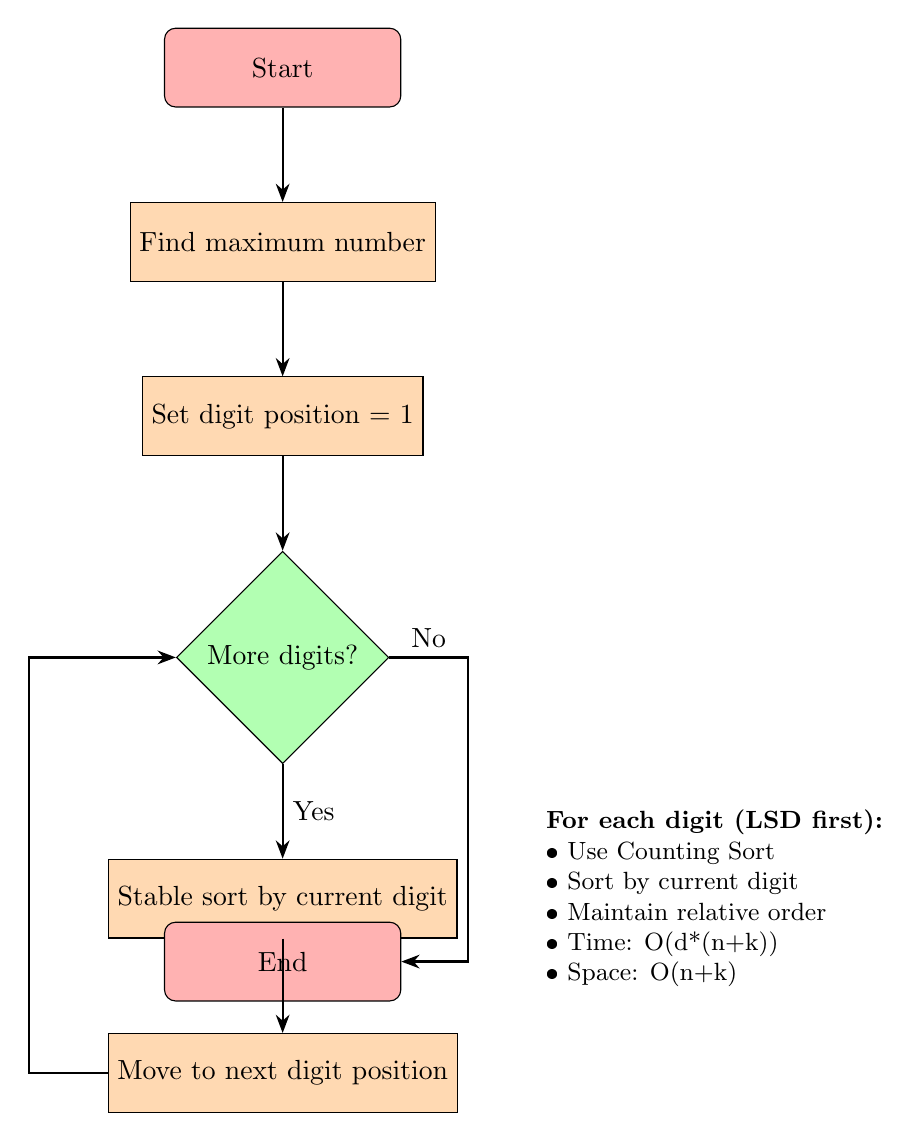
\begin{tikzpicture}[node distance=1.2cm]

\node (start) [startstop] {Start};
\node (findMax) [process, below=of start] {Find maximum number};
\node (initExp) [process, below=of findMax] {Set digit position = 1};
\node (dec1) [decision, below=of initExp] {More digits?};
\node (sortDigit) [process, below=of dec1] {Stable sort by current digit};
\node (nextDigit) [process, below=of sortDigit] {Move to next digit position};
\node (stop) [startstop, below=2cm of dec1] {End};

% Main flow
\draw [arrow] (start) -- (findMax);
\draw [arrow] (findMax) -- (initExp);
\draw [arrow] (initExp) -- (dec1);
\draw [arrow] (dec1) -- node[right] {Yes} (sortDigit);
\draw [arrow] (sortDigit) -- (nextDigit);
\draw [arrow] (nextDigit.west) -- ++(-1,0) |- (dec1.west);
\draw [arrow] (dec1.east) -- node[above] {No} ++(1,0) |- (stop.east);

% Algorithm details
\node [right=1cm of sortDigit, align=left, font=\small] {
    \textbf{For each digit (LSD first):}\\
    • Use Counting Sort\\
    • Sort by current digit\\
    • Maintain relative order\\
    • Time: O(d*(n+k))\\
    • Space: O(n+k)
};

\end{tikzpicture}
\end{document}
